\section{Web 2.0 - Abschlussarbeiten-DB}
Im Rahmen dieses Einführungsprojektes in gängige NoSQL ist ein relationales Schema gegeben, dass auf das jeweilige NoSQL äquivalent portiert werden soll. Zusätzlich sind Datensätze gegeben, die in den jeweiligen Datenbanken eingefügt werden sollen. 

\subsection{Das semantische Schema}
In der Abbildung \ref{fig:schema1} ist das Schema der Datenbank zu sehen, die in den gängigen NoSQL Techniken umgesetzt werden soll. Eine Abschlussarbeit wird von einem Studenten oder einem Auszubildenden geschrieben. In Auftrag gegeben wird die Arbeit von einer Organisation, die eine Universität oder ein Unternehmen sein kann. Die Arbeit wird eventuell von Erstprüfern und Zweitprüfern begutachtet. Der mit der Arbeit verbunden Abschluss hat einen Titel. Das Thema der Arbeit kann in einer Kategorie liegen, in der auch der Prüfer oder das Unternehmen liegen.\\

Insgesamt sind 27 Klassen gegeben, auf denen 36 Attribute verteilt sind. Im Zentrum des Schemas steht der Abschluss ("Degree"). Hier kommen alle wichtigen Informationen zusammen. \\

\begin{figure}[H]
	\centering
	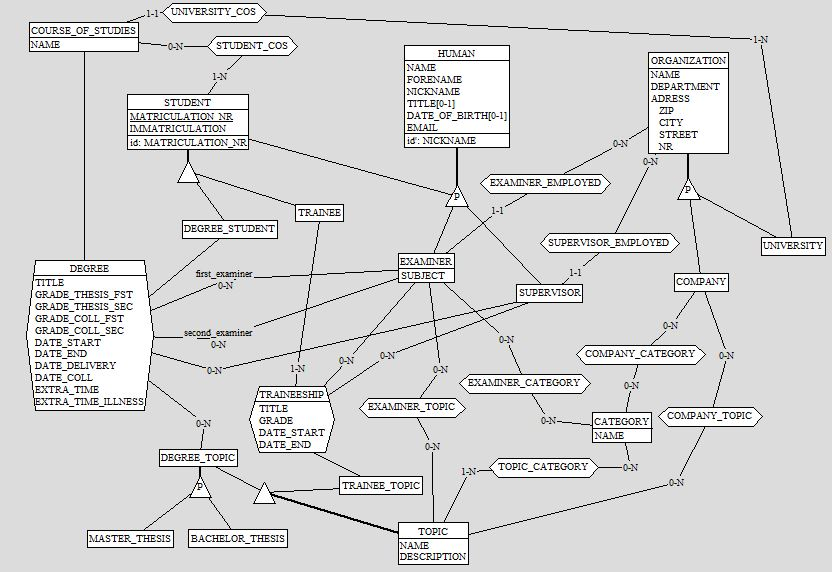
\includegraphics[scale=0.6]{images/01abschlussarbeitendbschema.jpg} 
	\caption{AbschlussarbeitenDB Schema}\label{fig:schema1}
\end{figure}

\subsection{Die Datenbestände}

\begin{figure}[H]
	\centering
	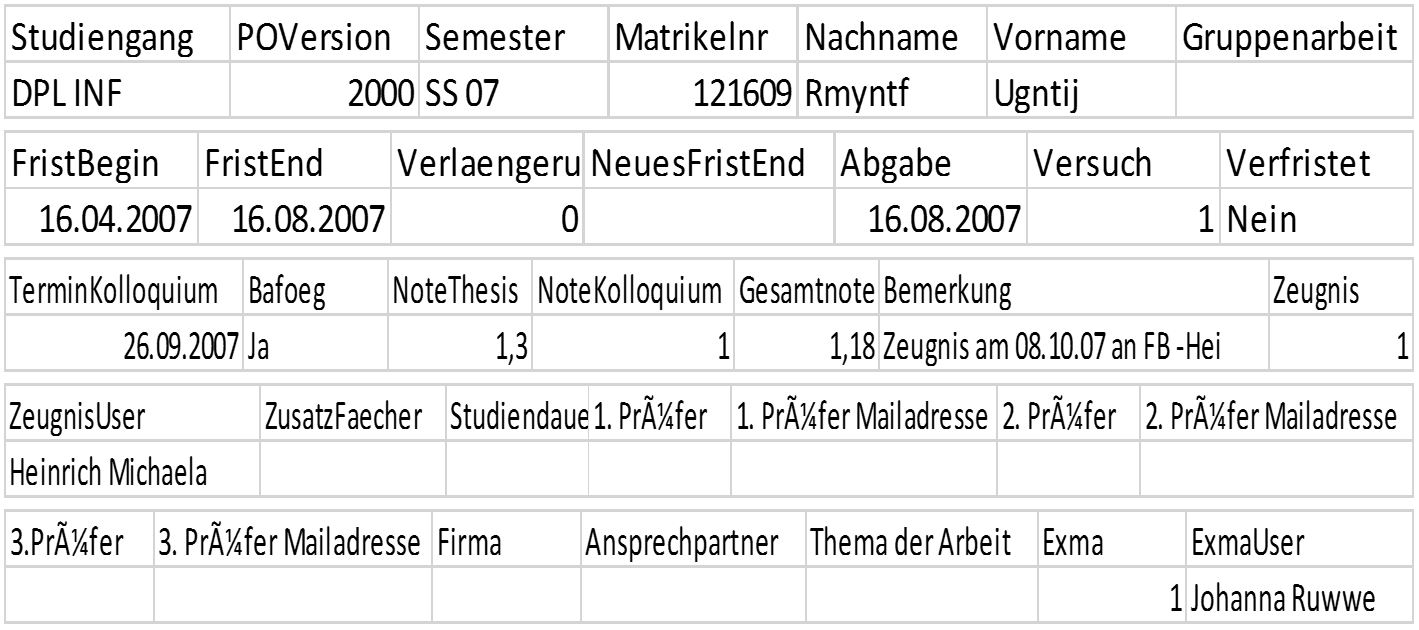
\includegraphics[scale=0.3]{images/01beispieldatensatzcsv.jpg} 
	\caption{Beispiel-Datensatz}\label{fig:schema2}
\end{figure}
